
Uit de twee simulaties zijn de volgende twee grafieken ontstaan. Figuur \ref{E1} is de grafiek die volgt uit de simulatie met enkele inverter en figuur \ref{E2} is ontstaan uit de simulatie met de drie inverters in cascade.
\\
In beide figuren zit de rode lijn Vin die de ingangsspanning voorsteld en de blauwe lijn Vout die de spanning gemeten over de belastingscapaciteit voorsteld. Deze ingangspanning gaat van 0V naar 5V(Maximale spanning) en andersom binnen 0,05s en heeft een periode van 0,4s.
\\
\\
Zoals je ziet in figuur \ref{E1} is de Vout lijn inderdaad geinverteerd in tegenstelling tot Vin zoals een inverter zich hoort te gedragen. De Vout lijn is alleen niet erg strak, bij elke overgang van 0V naar 5V is de Vout lijn rond de 5V afgerond en bij de overgang van 5V naar 0V is het rond de 0V afgerond.Deze ronding zijn ontstaan door het opladings en ontladings gedrag van een capaciteit, de capaciteit heeft namelijk tijd nodig om opgeladen te worden en om ontladen te worden.  
\\
In tegenstelling tot deze Vout lijn is de Vout lijn van figuur \ref{E2} bijna een perfecte blokgolf. Dit komt door het herstellende effect van inverters in cascade. Dit effect zorgt er namelijk voor dat, het Vin signaal al wordt geinverteerd voordat het signaal echt max spanning is. Het effect kan al een zwakke 0 inverteren naar een sterke 1, zo begint het opladen van de capaciteit veel eerder en zo wordt de Vout spanning meer lijkende op een blokgolf.  
\\ 
\\
Uit deze twee figuren kan de vertraging afgeleid worden voor de desbetreffende circuit oftwel de $t_{90\%}$ van het circuit. Uit figuur \ref{E1} kan afgelezen worden dat de vertraging van het circuit met enkele inverter 0,3 s is. 
\begin{figure} [h!]
\centering
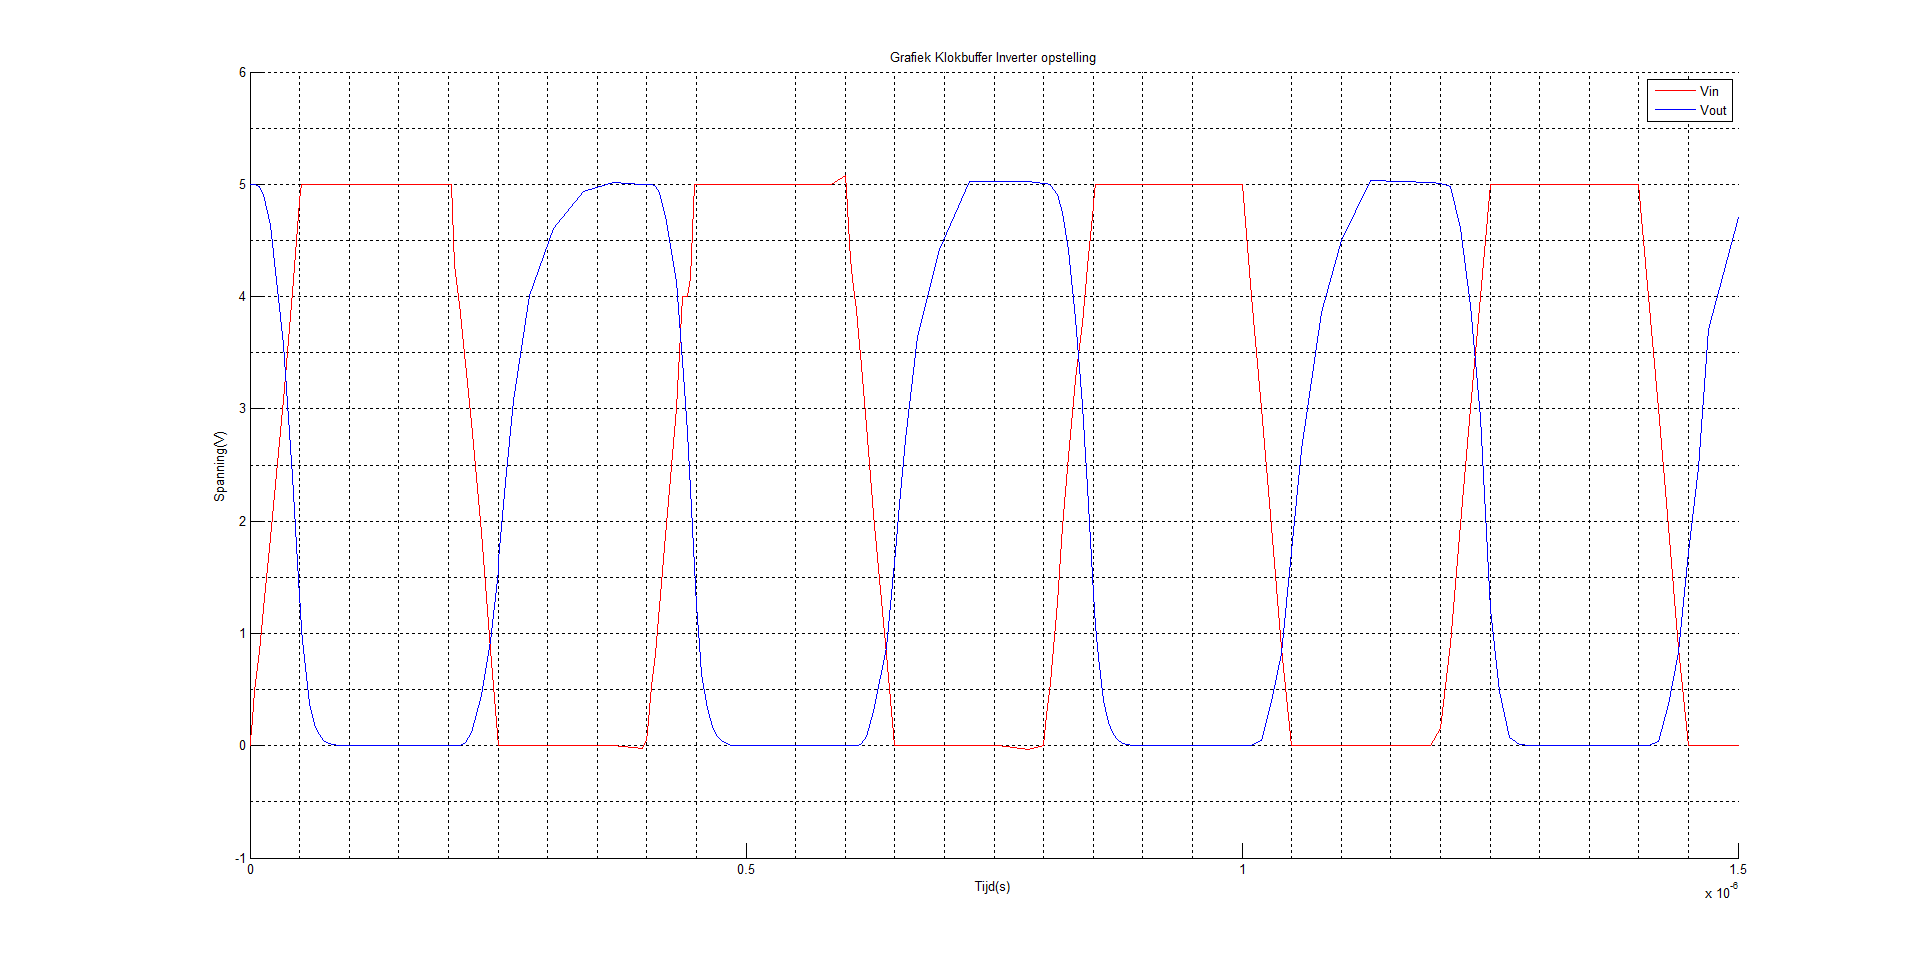
\includegraphics [width = \textwidth] {inputfiles/GrafiekInverter}
\caption{De simulatie resultaten van de enkele inverter in SPICE}
\label{E1}
\end{figure}
\\
Uit figuur \ref{E2} kan afgelezen worden dat de vertraging van het circuit met drie inverters in cascade 0,24 s is.

\begin{figure} [h!]
\centering
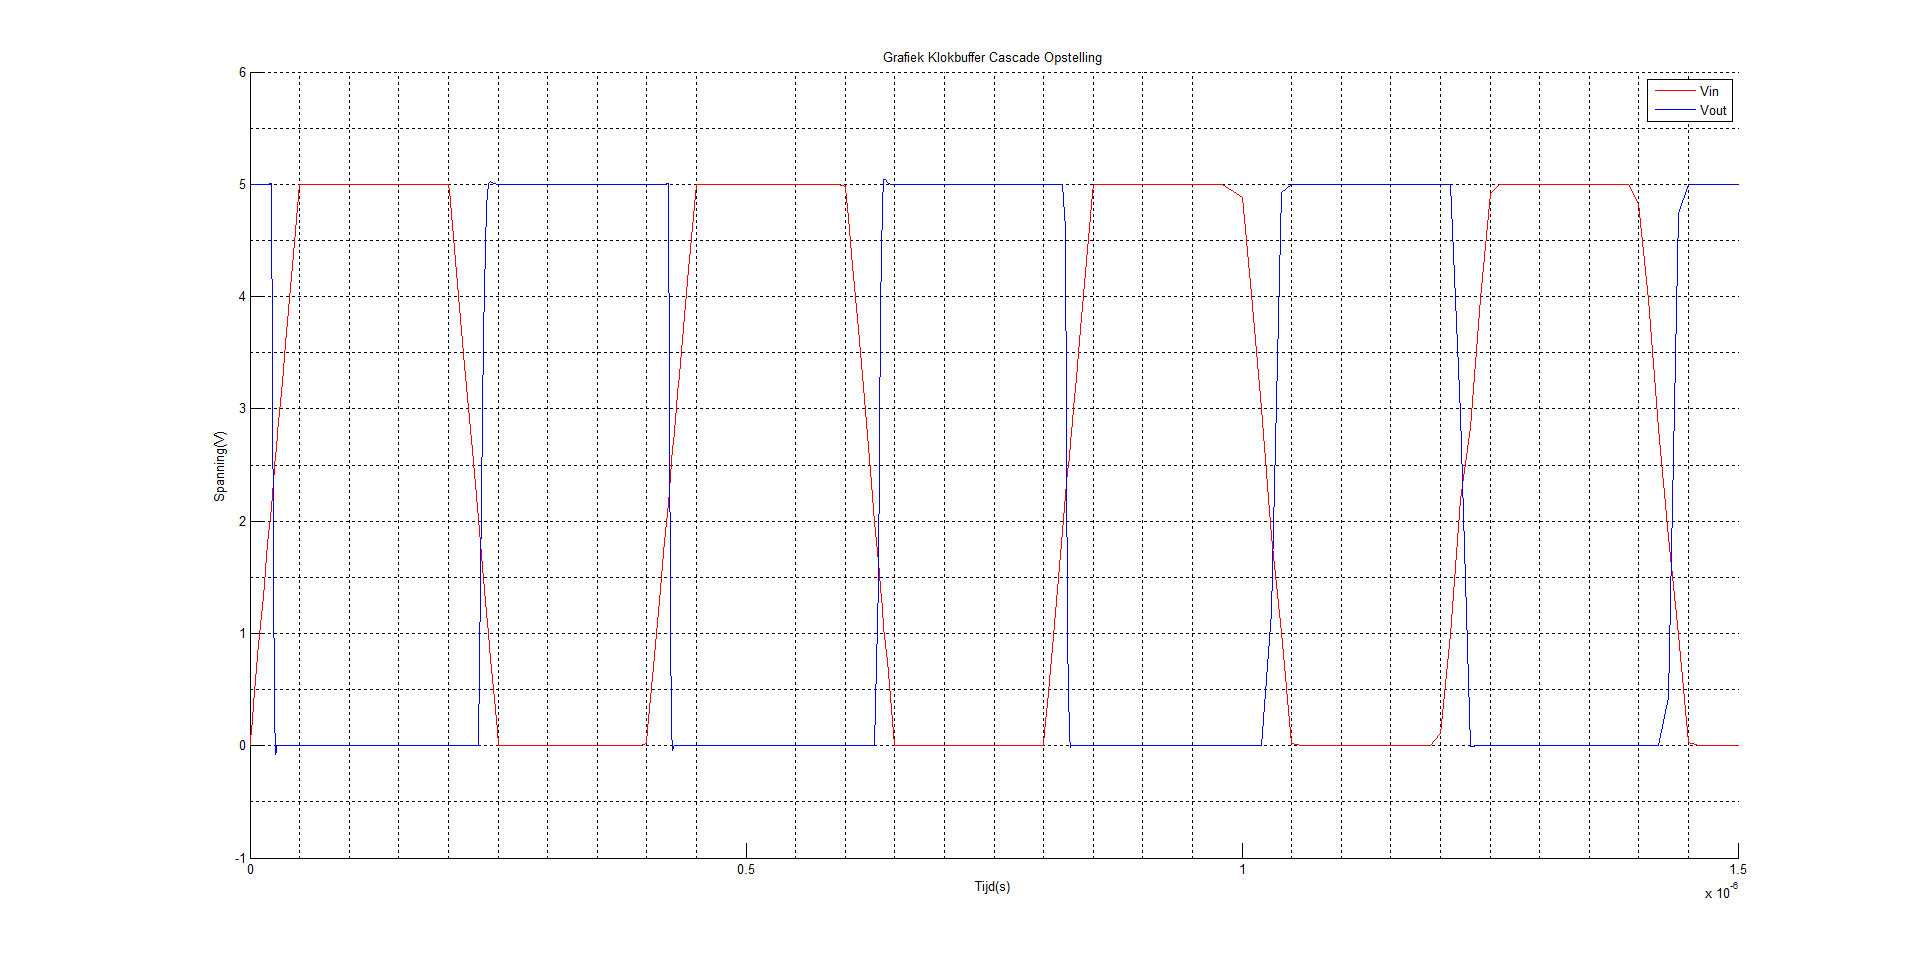
\includegraphics [width = \textwidth] {inputfiles/GrafiekCascade}
\caption{De simulatie resultaten van de driedubbele inverter in SPICE}
\label{E2}
\end{figure}

